\documentclass[journal,12pt,twocolumn]{IEEEtran}
\usepackage{setspace}
\usepackage{gensymb}
\singlespacing
\usepackage[cmex10]{amsmath}
\usepackage{amsthm}
\usepackage{mathrsfs}
\usepackage{txfonts}
\usepackage{stfloats}
\usepackage{bm}
\usepackage{cite}
\usepackage{cases}
\usepackage{subfig}
\usepackage{longtable}
\usepackage{multirow}
\usepackage{enumitem}
\usepackage{mathtools}
\usepackage{steinmetz}
\usepackage{tikz}
\usepackage{circuitikz}
\usepackage{verbatim}
\usepackage{tfrupee}
\usepackage[breaklinks=true]{hyperref}
\usepackage{tkz-euclide}
\usetikzlibrary{calc,math}
\usepackage{listings}
    \usepackage{color}                                            %%
    \usepackage{array}                                            %%
    \usepackage{longtable}                                        %%
    \usepackage{calc}                                             %%
    \usepackage{multirow}                                         %%
    \usepackage{hhline}                                           %%
    \usepackage{ifthen}                                           %%
  %optionally (for landscape tables embedded in another document): %%
    \usepackage{lscape}     
\usepackage{multicol}
\usepackage{chngcntr}
\DeclareMathOperator*{\Res}{Res}
\renewcommand\thesection{\arabic{section}}
\renewcommand\thesubsection{\thesection.\arabic{subsection}}
\renewcommand\thesubsubsection{\thesubsection.\arabic{subsubsection}}

\renewcommand\thesectiondis{\arabic{section}}
\renewcommand\thesubsectiondis{\thesectiondis.\arabic{subsection}}
\renewcommand\thesubsubsectiondis{\thesubsectiondis.\arabic{subsubsection}}

% correct bad hyphenation here
\hyphenation{op-tical net-works semi-conduc-tor}
\def\inputGnumericTable{}                                 %%

\lstset{
frame=single, 
breaklines=true,
columns=fullflexible
}

\begin{document}


\newtheorem{theorem}{Theorem}[section]
\newtheorem{problem}{Problem}
\newtheorem{proposition}{Proposition}[section]
\newtheorem{lemma}{Lemma}[section]
\newtheorem{corollary}[theorem]{Corollary}
\newtheorem{example}{Example}[section]
\newtheorem{definition}[problem]{Definition}
\newcommand{\BEQA}{\begin{eqnarray}}
\newcommand{\EEQA}{\end{eqnarray}}
\newcommand{\define}{\stackrel{\triangle}{=}}

\bibliographystyle{IEEEtran}
\providecommand{\mbf}{\mathbf}
\providecommand{\pr}[1]{\ensuremath{\Pr\left(#1\right)}}
\providecommand{\qfunc}[1]{\ensuremath{Q\left(#1\right)}}
\providecommand{\sbrak}[1]{\ensuremath{{}\left[#1\right]}}
\providecommand{\lsbrak}[1]{\ensuremath{{}\left[#1\right.}}
\providecommand{\rsbrak}[1]{\ensuremath{{}\left.#1\right]}}
\providecommand{\brak}[1]{\ensuremath{\left(#1\right)}}
\providecommand{\lbrak}[1]{\ensuremath{\left(#1\right.}}
\providecommand{\rbrak}[1]{\ensuremath{\left.#1\right)}}
\providecommand{\cbrak}[1]{\ensuremath{\left\{#1\right\}}}
\providecommand{\lcbrak}[1]{\ensuremath{\left\{#1\right.}}
\providecommand{\rcbrak}[1]{\ensuremath{\left.#1\right\}}}
\theoremstyle{remark}
\newtheorem{rem}{Remark}
\newcommand{\sgn}{\mathop{\mathrm{sgn}}}
\providecommand{\abs}[1]{\left\vert#1\right\vert}
\providecommand{\res}[1]{\Res\displaylimits_{#1}} 
\providecommand{\norm}[1]{\left\lVert#1\right\rVert}
\providecommand{\mtx}[1]{\mathbf{#1}}
\providecommand{\mean}[1]{E\left[ #1 \right]}
\providecommand{\fourier}{\overset{\mathcal{F}}{ \rightleftharpoons}}
\providecommand{\system}{\overset{\mathcal{H}}{ \longleftrightarrow}}
\newcommand{\solution}{\noindent \textbf{Solution: }}
\newcommand{\cosec}{\,\text{cosec}\,}
\providecommand{\dec}[2]{\ensuremath{\overset{#1}{\underset{#2}{\gtrless}}}}
\newcommand{\myvec}[1]{\ensuremath{\begin{pmatrix}#1\end{pmatrix}}}
\newcommand{\mydet}[1]{\ensuremath{\begin{vmatrix}#1\end{vmatrix}}}
\numberwithin{equation}{subsection}
\makeatletter
\@addtoreset{figure}{problem}
\makeatother

\let\StandardTheFigure\thefigure
\let\vec\mathbf
\renewcommand{\thefigure}{\theproblem}



\def\putbox#1#2#3{\makebox[0in][l]{\makebox[#1][l]{}\raisebox{\baselineskip}[0in][0in]{\raisebox{#2}[0in][0in]{#3}}}}
     \def\rightbox#1{\makebox[0in][r]{#1}}
     \def\centbox#1{\makebox[0in]{#1}}
     \def\topbox#1{\raisebox{-\baselineskip}[0in][0in]{#1}}
     \def\midbox#1{\raisebox{-0.5\baselineskip}[0in][0in]{#1}}

\vspace{3cm}


\title{Assignment 1}
\author{Jaswanth Chowdary Madala}





% make the title area
\maketitle

\newpage

%\tableofcontents

\bigskip

\renewcommand{\thefigure}{\theenumi}
\renewcommand{\thetable}{\theenumi}


\begin{enumerate}
\item If a line intersects two concentric circles (circles
with the same centre) with centre $\vec{O}$ at $\vec{A}$, $\vec{B}$, $\vec{C}$ and $\vec{D}$, prove that $AB = CD$.
\begin{figure}[ht]
\centering
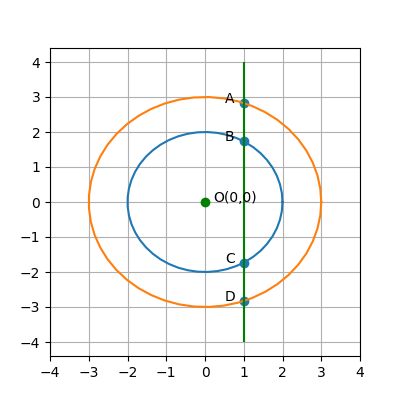
\includegraphics[width = \columnwidth]{figs/fig.png}
\caption{Graph}
\label{fig:1}
\end{figure}

\textbf{Solution:}
Let the equations of two concentric circles be,
\begin{align}
\norm{\vec{x}}^2 &= 4
\label{eq:1}\\
\norm{\vec{x}}^2 &= 9
\label{eq:2}
\end{align}

The line should intersect both the circles i.e., distance between the line and the center of circle should be less than the radius of smaller circle. Let the equation of the line be,
\begin{align}
\vec{x} &= \vec{h} + \mu \vec{m}
\end{align}
The normal vector of this line is given by,
\begin{align}
\vec{n} &= \myvec{0&-1\\1&0}\vec{m}
\end{align}
The equation of the line is given by,
\begin{align}
\vec{n}^\top\vec{x} - \vec{n}^\top\vec{h} = 0
\end{align}
The distance between origin and line is given by,
\begin{align}
d &= \frac{\abs{\vec{n}^\top\vec{h}}}{\norm{\vec{n}}}
\end{align}
The condition for intersection is
\begin{align}
d < 2
\end{align}
Consider
\begin{align}
\vec{h} = \myvec{1\\0}, \, \vec{m} &= \myvec{0\\1}
\end{align}
then we get the distance as,
\begin{align}
\vec{n} &= \myvec{-1\\0}\\
d &= 1
\end{align}
Hence, the taken parameters $\vec{h}, \vec{m}$ satisfies the reqiuired conditions.

The parameter $\mu$ of the points of intersection of line \eqref{eq:4} with the conic section \eqref{eq:5}
\begin{align}
\vec{x} &= \vec{h} + \mu \vec{m}
\label{eq:4}\\
\text{g}\brak{\vec{x}} &= \vec{x}^{\top}\vec{V}\vec{x}+2\vec{u}^{\top}\vec{x}+f=0
\label{eq:5}
\end{align}
is given by the equation 
\begin{align}
\mu^2\vec{m}^{\top}\vec{V}\vec{m} + 2 \mu\vec{m}^{\top}\brak{\vec{V}\vec{h}+\vec{u}} 
	+ \text{g}\brak{\vec{h}} &=0
\label{eq:6}
\end{align}


The points of intersection of circle \eqref{eq:1} and the line \eqref{eq:4} $\vec{B},\vec{C}$ are given by,
\begin{align}
\vec{V} = \vec{I}, \, \vec{u} = \vec{O}, \, f &= -4
\label{eq:7}\\
\vec{h} = \myvec{1\\0}, \, \vec{m} &= \myvec{0\\1}
\label{eq:8}
\end{align} 
Substituting the above expressions \eqref{eq:7}, \eqref{eq:8} in \eqref{eq:6}, we get
\begin{align}
\vec{m}^{\top}\vec{V}\vec{m} & = 1\\
\vec{m}^{\top}\brak{\vec{V}\vec{h}+\vec{u}} &= 0 \\
\text{g}\brak{\vec{h}} &= -3\\
\mu ^2 - 3 &= 0\\
\mu &= \pm \sqrt{3}\\
\vec{B} = \myvec{1\\\sqrt{3}}, \, \vec{C} &= \myvec{1\\-\sqrt{3}}
\end{align}

The points of intersection of circle \eqref{eq:2} and the line \eqref{eq:4} $\vec{A},\vec{D}$ are given by,
\begin{align}
\vec{V} = \vec{I}, \, \vec{u} = \vec{O}, \, f &= -9
\label{eq:9}\\
\vec{h} = \myvec{1\\0}, \, \vec{m} &= \myvec{0\\1}
\label{eq:10}
\end{align} 
Substituting the above expressions \eqref{eq:9}, \eqref{eq:10} in \eqref{eq:6}, we get
\begin{align}
\vec{m}^{\top}\vec{V}\vec{m} & = 1\\
\vec{m}^{\top}\brak{\vec{V}\vec{h}+\vec{u}} &= 0 \\
\text{g}\brak{\vec{h}} &= -8\\
\mu ^2 - 8 &= 0\\
\mu &= \pm 2\sqrt{2}\\
\vec{A} = \myvec{1\\2\sqrt{2}}, \, \vec{D} &= \myvec{1\\-2\sqrt{2}}
\end{align}

\begin{align}
\norm{\vec{A}-\vec{B}} &= \norm{\myvec{0 \\ 2\sqrt{2}-\sqrt{3}}}\\
&=  2\sqrt{2}-\sqrt{3}\\
\norm{\vec{C}-\vec{D}} &= \norm{\myvec{0 \\ 2\sqrt{2}-\sqrt{3}}}\\
&=  2\sqrt{2}-\sqrt{3}
\end{align}
Hence $AB = CD$.
The parameters used in the construction are shown in the below table \ref{tab:1}

\begin{table}[h]
\centering
%%%%%%%%%%%%%%%%%%%%%%%%%%%%%%%%%%%%%%%%%%%%%%%%%%%%%%%%%%%%%%%%%%%%%%
%%                                                                  %%
%%  This is a LaTeX2e table fragment exported from Gnumeric.        %%
%%                                                                  %%
%%%%%%%%%%%%%%%%%%%%%%%%%%%%%%%%%%%%%%%%%%%%%%%%%%%%%%%%%%%%%%%%%%%%%%

\begin{center}
\begin{tabular}{|c|c|c|}
\hline
\textbf{RV}& \textbf{Values} & \textbf{Description} \\ \hline
$X$		   & 	$\{0,1\}$	&  1st draw - 0: black card, 1: red card\\ \hline
$Y$ 		   & 	$\{0,1\}$	&  2nd draw - 0: black card, 1: red card\\ \hline
$X,Y$ 		   & 	$\{00\}$	&	2 cards drawn are black\\ \hline
\end{tabular}
\end{center}

\caption{}
\label{tab:1}
\end{table}
\end{enumerate}
\end{document}